\chapter{Process Description Language Grammar}
\label{chp:grammar}

\section{Overview}

One of the goals of \SBGNPDLone is to provide a visual description of biological systems that can accurately and unambiguously  convey to the reader what the writer of a \PDm meant. A secondary, but nevertheless important goal is to provide a visual language that can be supported by software tools. To achieve both goals we require a detailed set of rules that are universally applied to \PDms. In \chap{glyphs} the glyphs of the \PDl were introduced and key usage rules were described; we expect that this will be sufficient for casual users of the notation. However, this chapter provides a more detailed description of the rules that apply to the \PDl and it is anticipated that this will be required reading for advanced users of the notation and tool developers implementing SBGN \PD viewers or editors.

In addition to understanding the rules of the notation it is also important to understand the underlying model, or abstraction, of the biological world that the \PDl uses. By understanding the abstractions used one can also understand more clearly what the author of a map meant, and also what the author could not say given the limitations of the notation. In the next section, we describe the abstractions and concepts implicit in the SBGN \PDl.

\section{Concepts}
\label{sec:concepts}

The key abstraction of the SBGN \PDl is one of  processes that act on pools of entities. The entities are typically biological molecules, but need not be (such as a \glyph{perturbing agent}), and the \glyph{process} is typically a combination of one or more  biochemical reactions, but again need not be.
Processes are controlled, or \emph{modulated}, by other entity pools and new entities can be obtained from an \glyph{empty set} and existing entities discarded to an \glyph{empty set}.

It can be helpful to think of the SBGN \PD as describing the flow of a fluid, especially when trying to understand concepts such as stoichiometry, and modulation. In this analogy, each \glyph{EPN} represents a tank of fluid, which may be emptied via a pipe (the consumption arc, \sect{consumption}) that is connected to a valve (the process node, \sect{PNs}), which in turn is connected to other pipes (the production arcs, \sect{production}) that fill other tanks (\glyph{EPNs}). The opening of the valve, and thus the rate of the process can be controlled by the volume of fluid in another tank (this is modulation)\footnote{The precise nature of the relationship between valve opening and amount of fluid determines the nature of the modulation.}. If there are two consumption pipes feeding fluid into the process and one is wider and allows double the flow of the first then the fluid will mix in the process with a 2:1 ratio. This corresponds to the stoichiometry of the \glyph{consumption} and \glyph{production} arcs. Finally, the system needs a source of fluid from one or more external sources (represented with the \glyph{empty set}, see section \sect{emptySet}) and one or more sinks for it to drain away (also represented with the \glyph{empty set}).

One can see that this maps very closely to the abstraction described in the \PDl, but it also has an interesting side-effect that it allows us to add quantities to SBGN glyphs. In particular, EPNs have an implicit amount of entities in the entity pool and processes have an implicit rate. Since SBGN \PD is not a modelling language this will not be discussed in any further detail, however, this is an important concept that underpins our understanding of how processes are modulated in \sect{mod-semantics}.

\section{The conceptual model}
\label{sec:conceptual-model}

In order to formalize the conceptual representation described above and the glyph specific rules that we will describe later, we have described the \PDl using UML Domain Object Model. We have used it to define the ``taxonomy'' of the \PD glyphs and their relationship to each other. Finally we describe the attributes of each node glyph that are required to uniquely identify an instance of it in a \PDm. The concept of identity is important in some of the rules described below.

\begin{figure}[htb]
\begin{center}
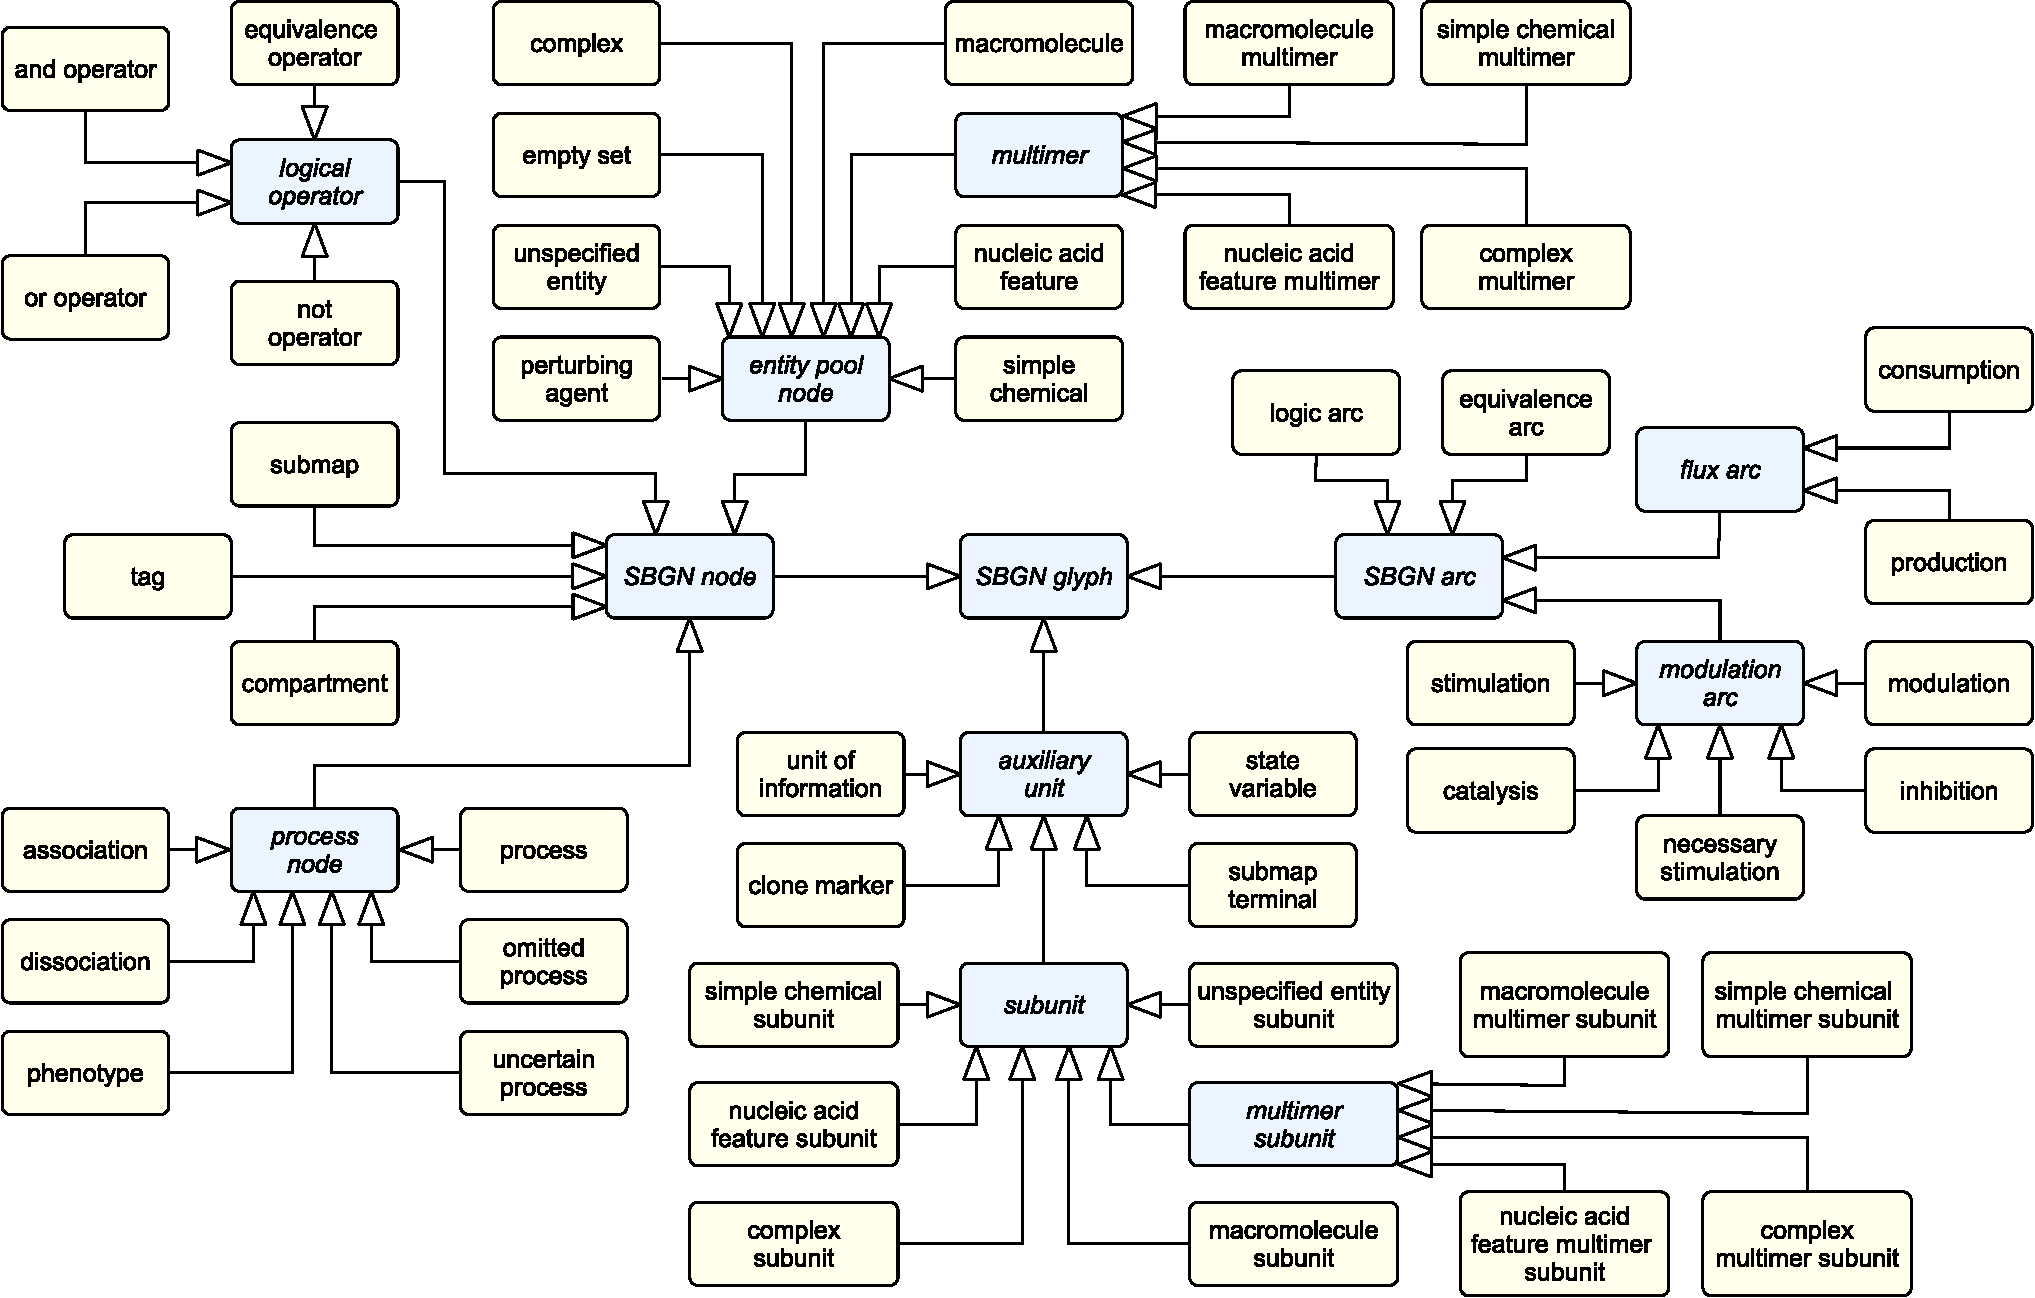
\includegraphics[width=\linewidth]{images/build/sbgn_glyph_model.pdf}
\caption{Organisation of the node, arc and auxiliary unit glyphs within SBGN \PDl. All UML classes (boxes) correspond to \PD glyphs except those with italicised names, which are organisational groupings. They correspond to the groupings used elsewhere in this document.}
\label{fig:sbgn_node_tax}
\end{center}
\end{figure}


\begin{center}
\begin{small}
\tablefirsthead{\hline
\textbf{Glyph} & \textbf{Identifying Attributes} \\\hline}
\tablehead{\hline
\multicolumn{2}{|l|}{\small\sl continued from previous page}\\\hline
\textbf{Glyph} & \textbf{Identifying Attributes} \\\hline\hline}
\tabletail{\hline
\multicolumn{2}{|r|}{\small\sl continued on next page}\\
\hline}
\tablelasttail{\hline}

\topcaption{The Identifying attributes of \PD node glyphs. When a glyph is always unique in a map, this is indicated by the term \emph{instance}. The term \emph{state values} indicates that the values of all the EPN's state variables are used in the definition of its identity.}

\pagebreak
\begin{supertabular}{|p{4.5cm}|p{10cm}|}\hline
Unit of Information & \emph{instance} \\\hline
State variable & Owning StatefulEpnNode, value \\\hline

Clone maker & Owning EpnNode \\\hline
Labelled clone maker & Owning EpnNode, Label \\\hline
Unspecified entity & Owning compartment, Label \\\hline
Simple chemical & Owning compartment, Label \\\hline
Macromolecule & Owning compartment, Label, Material type, \emph{state values} \\\hline
Nucleic acid feature & Owning compartment, Label, Conceptual type, \emph{state values} \\\hline
Complex & Owning compartment, Label,  \emph{state values} \\\hline
Simple chemical multimer & Owning compartment, Label, Cardinality \\\hline
Macromolecule multimer & Owning compartment, Label, Material type, Cardinality, \emph{state values} \\\hline
Nucleic acid feature multimer & Owning compartment, Label, Conceptual type, Cardinality, \emph{state values} \\\hline
Complex multimer & Owning compartment, Label, Cardinality,  \emph{state values} \\\hline
Empty set & \emph{instance} \\\hline
Perturbing agent & Label \\\hline
Tag & Label \\\hline
Submap terminal & Label \\\hline
Compartment & Label \\\hline
Submap & Label \\\hline
Process & \emph{instance} \\\hline
Omitted process & \emph{instance} \\\hline
Uncertain process & \emph{instance} \\\hline
Association & \emph{instance} \\\hline
Dissociation & \emph{instance} \\\hline
Phenotype & \emph{instance} \\\hline
\end{supertabular}
\end{small}
\end{center}


\paragraph*{Notes}

A complex may have a Label or be defined by its subunits. In the case where it has both then all complexes with the same label must also have the same subunit composition.

\section{Syntax}

The syntax of the SBGN \PDl is defined in the form of an incidence matrix. An incidence matrix has arcs as rows and nodes as columns. Each element of the matrix represents the role of an arc in connection to a node. Source (S) means that the arc can begin at that node. Target (T) indicates that the arc can end at that node. Numbers in parenthesis represent the maximum number of arcs of a particular type to have this specific connection role with the node. Empty cells means the arc is not able to connect to the node.

\subsection{Node connectivity}

\begin{center}
\begin{tabular}{||c|c|c|c|c|c|c|c|c|c|c|c|c||}
\hline
\hline
\raisebox{20pt}{$Arc \backslash EPN$} &\vglyph{macromolecule} & \vglyph{simple chemical} & 
\vglyph{unspecified entity} &  \vglyph{multimer} & \vglyph{complex} & 
\vglyph{nucleic acid feature}& \vglyph{tag} & \vglyph{submap terminal} & \vglyph{empty set} & 
\vglyph{perturbing agent} &  \vglyph{submap}\\ \hline 
\glyph{consumption}      & S & S & S & S & S & S &   & & S(1) &  & \\ \hline 
\glyph{production}        & T & T & T & T & T & T &   & & T(1) &  & \\ \hline 
\glyph{modulation}        & S & S & S & S & S & S &   & &  & S & \\ \hline 
\glyph{stimulation}        & S & S & S & S & S & S &   & & & S & \\ \hline 
\glyph{catalysis}          & S & S & S & S & S &   &   & & &   & \\ \hline 
\glyph{inhibition}          & S & S & S & S & S & S &   & & & S & \\ \hline 
\glyph{necessary stimulation} & S & S & S & S & S & S &  & &  & S & \\ \hline 
\glyph{logic arc}          & S & S & S & S & S & S &   &  & &   & \\ \hline 
\glyph{equivalence arc}     & S & S & S & S & S & S & T & T  & & \\ \hline \hline
\end{tabular}
\end{center}

\paragraph*{Additional rules}

\begin{enumerate}
    \item An EPN that is a \glyph{subunit} of a \glyph{complex} can only be linked to a modulation arc.
    \item With the above exception, glyphs that are subunits cannot be connect to any arc glyph.
    \item A \glyph{logic arc} that is linked to an \glyph{equivalence operator} on one side can only be linked to an EPN on the other side.
\end{enumerate}
    
\begin{center}
\begin{tabular}{||c|c|c|c|c|c|c|c|c|c|c||}
\hline
\hline
\raisebox{20pt}{$Arc \backslash PN$} & \vglyph{process}  & \vglyph{omitted process}  & 
\vglyph{uncertain process} & \vglyph{phenotype}  & \vglyph{association}  & \vglyph{dissociation}  & \vglyph{and}  &  
\vglyph{or} & \vglyph{not} & \vglyph{equivalence} \\ \hline 
\glyph{consumption} & T & T &  T & & T    & T(1)\footnotemark[1] &      &      &  &    \\ \hline
\glyph{production}  & S & S & S & & S(1)\footnotemark[1] & S    &      &      &   &   \\ \hline
\glyph{modulation}  & T & T & T & T  & T  &   T  & S(1) & S(1) & S(1) & \\ \hline
\glyph{stimulation} & T & T & T & T & T  &   T  & S(1) & S(1) & S(1) & \\ \hline
\glyph{catalysis}   & T & T & T & T & T  &  T   & S(1) & S(1) & S(1) & \\ \hline
\glyph{inhibition}  & T & T & T &  T & T  &   T  & S(1) & S(1) & S(1) & \\ \hline
\glyph{necessary stimulation}     & T & T & T &  T &  T &  T   & S(1) & S(1) & S(1) & \\ \hline
\glyph{logic arc}   &   &   &   &      & &      & \begin{tabular}{@{}c@{}}S(1) \\ T\end{tabular}    & \begin{tabular}{@{}c@{}}S(1) \\ T\end{tabular}    & \begin{tabular}{@{}c@{}}S(1) \\ T(1)\end{tabular} & \begin{tabular}{@{}c@{}}S(1) \\ T\end{tabular} \\ \hline
\glyph{equivalence arc} &   &   &  &    & &      &      &      &    &  \\ \hline \hline
\end{tabular}
\footnotetext[1]{The cardinality restriction is deprecated in this version.}
\end{center}

\subsection{Containment definition}
\label{sec:containment}

By containment we mean that a glyph can be drawn inside the other glyph. This does not necessarily mean that the glyph ``belongs'' the the containing node, although in some cases it does. In this section the concept of ``belonging'' is referred to as ownership and you can find node ownership in \sect{conceptual-model}. There are two glyphs that allow containment: \glyph{compartment} and \glyph{complex}. The next table describes the relationship between \PD glyphs and these containers. A $+$ means that the element may be drawn within a container. A $-$ means containment is not allowed.

\begin{center}
\tablefirsthead{\hline
\textbf{Glyph $\backslash$ Containers}  & \textbf{\glyph{complex}} & \textbf{\glyph{compartment}}  \\\hline\hline}
\tablehead{\hline
\multicolumn{3}{|l|}{\small\sl continued from previous page}\\\hline
\textbf{Glyph $\backslash$ Containers}  & \textbf{\glyph{complex}} & \textbf{\glyph{compartment}}  \\\hline\hline}
\tabletail{\hline
\multicolumn{3}{|r|}{\small\sl continued on next page}\\
\hline}
\tablelasttail{\hline}

\begin{supertabular}{|c|c|c|}
\glyph{unspecified entity}    &         +       &          +         \\ \hline
\glyph{simple chemical}      &         +       &          +         \\ \hline
\glyph{macromolecule}        &         +       &          +        \\ \hline
\glyph{nucleic acid feature}   &         +       &          +      \\ \hline 
\glyph{multimer}             &         +       &          +         \\ \hline
\glyph{empty set}          &         -       &          +          \\ \hline 
\glyph{perturbing agent}          &         -       &          +      \\ \hline
\glyph{phenotype}           &         -       &          +         \\ \hline
\glyph{tag}                  &         -       &          +          \\ \hline
\glyph{submap terminal}    &         -       &   +         \\ \hline
\glyph{state variable}    &         +       &   +               \\ \hline
\glyph{complex}              &         +       &          +       \\ \hline
\glyph{compartment}          &         -       &          +      \\ \hline
\glyph{submap}               &         -       &          +         \\ \hline
\glyph{process}             &         -       &          +         \\ \hline
\glyph{omitted process}      &         -       &          +     \\ \hline
\glyph{uncertain process}    &         -       &          +        \\ \hline
\glyph{association}          &         -       &          +         \\ \hline
\glyph{dissociation}         &         -       &          +         \\ \hline
\glyph{consumption}          &         -       &          +        \\ \hline
\glyph{production}           &         -       &          +          \\ \hline
\glyph{modulation}           &         -       &          +         \\ \hline
\glyph{stimulation}          &         -       &          +          \\ \hline
\glyph{catalysis}            &         -       &          +          \\ \hline
\glyph{inhibition}           &         -       &          +         \\ \hline
\glyph{necessary stimulation}   &         -       &          +     \\ \hline
\glyph{logic arc}            &         -       &          +          \\ \hline
\glyph{equivalence arc}      &         -       &          +      \\ \hline
\glyph{and}                  &         -       &          +         \\ \hline
\glyph{or}                   &         -       &          +          \\ \hline
\glyph{not}                  &         -       &          +         \\ \hline
\glyph{equivalence}                  &         -       &          +         \\ \hline
\hline
\end{supertabular}
\end{center}


\section{Semantic rules}

\subsection{EPNs}

 \begin{enumerate}
   \item All \glyph{state variables} associated with a Stateful Entity Pool Node should be unique and not duplicated within that node.
   \item If a state variable is used in one EPN then is must be used in all equivalent stateful EPNs\footnote{A stateful EPN is equivalent if the EPNs are identical when their state descriptions are ignore.}.
   \item EPNs should not be orphaned (i.e.\, they must be associated with at least one arc.
%    \item A \glyph{complex} should consists of different EPNs. If two or more 
%    elements of the complex are identical they should be replaced by multimer. 
 \end{enumerate}

\subsection{Process Nodes}

As described in \sect{process}, the \glyph{consumption} and \glyph{production} arcs converge before connecting to the process node (\fig{process-sidedness}). This defines the EPNs that are the input and outputs of an irreversible process. Since, processes can be reversible in the following rules we refer to these groupings as the ``left-hand-side'' (LHS) and ``right-hand-side'' (RHS) of the process\footnote{Note this designation is purely for grouping and is used even then the sides of the reaction are above and below the process.}. For convenience we will also collectively refer to the \glyph{consumption} and \glyph{production} arcs as \emph{flux} arcs.

\begin{figure}[H]
  \centering
  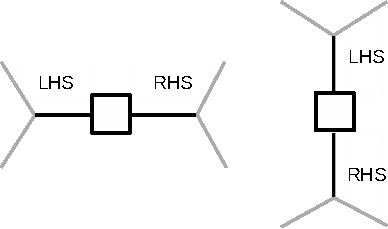
\includegraphics[scale = 0.4]{images/process_sidedness}
  \caption{An illustration of the ``sidedness'' of a process. The designation of LHS and RHS is essentially arbitrary.}
  \label{fig:process-sidedness}
\end{figure}

\subsubsection{Flux Arcs}

\begin{enumerate}
\item All process nodes (with the exception of \glyph{phenotype}) must have a LHS and RHS.
    \item All EPNs on the LHS of a process must be unique.
    \item All EPNs on the RHS of a process must be unique.
    \item All \glyph{phenotype} glyphs must be associated with at least one modulation arc.
    \item The EPNs that make up the LHS of the process should be consistent with the RHS, i.e.\, the process should constitute a    balanced biochemical reaction.
    \item Once the stoichiometry of a flux arc is displayed in a map then all other flux arcs should
    display theit stoichiometry make.
    \item If the stoichiometry is undefined or unknown this should be indicated by the use of a question mark (``?''). 
   \item If more than one set of stoichiometries can be applied to the flux arcs of the process then the stoichiometry of the flux arcs must be displayed.
%     \item \glyph{PNs} should have only one \glyph{Catalysis} arc connected to them. If
%     there more than one catalyst known to affect the process, several \glyph{PNs} should be
%     drawn or a \glyph{logical operator} used 
%     \item \glyph{PNs} should have only one \glyph{necessary stimulation} arc connected to it. If
%     there is more than one \glyph{EPN} acting as a necessary stimulator on a process, then a \glyph{logic operator} should be used.
\end{enumerate}  

\subsubsection{\glyph{Association}}

  \begin{enumerate}
    \item An \glyph{Association} is always an irreversible process.
\end{enumerate}  

\subsubsection{\glyph{Dissociation}}
  \begin{enumerate}
    \item An \glyph{Dissociation} is always an irreversible process.
\end{enumerate}  

\subsubsection{Modulation}
\label{sec:mod-semantics}

As discussed in \sect{concepts}, it is implied, but not defined explicitly that the process has a rate at
which it converts its LHS EPNs to its RHS EPNs (and vice-versa in the case of a reversible process). This concept is
important in understanding how the \PDl describes process modulation.

\begin{enumerate}
\item A \glyph{process} with no modulations has an underlying ``basal rate''
  which describes the rate at which it converts inputs to outputs.
\item A \glyph{modulation} changes the basal rate in an unspecified fashion.
\item A \glyph{stimulation} is a modulation that increases the basal rate.
\item An \glyph{inhibition} is a modulation that decreases the basal rate.
\item The above types of modulation, when assigned to the same process, are combined and have a multiplicative effect on the basal rate of the process.
\item Modulators that do not interact with each other in the above manner, should be drawn as modulating different process nodes. Their effect is therefore additive.
\item At most one \glyph{necessary stimulation} can be assigned to a process node. Two \glyph{necessary stimulations}
  would imply an implicit AND or OR operator. For clarity only
  one \glyph{necessary stimulation} can be assigned to a \glyph{process}, and such combinations must be
  explicitly expressed using \glyph{logical operators}.  \item At most one \glyph{catalysis} can be assigned to a \glyph{process}. A catalysis arcs
  modulation implies that the exact biochemical mechanism underlying
  the process is known. In this context two \glyph{catalysis} cannot
  be assigned to the same process node as they represent
  independent reactions. Other EPNs can be
  assigned to the same process than a catalysis, such as modulators, stimulators, and
  inhibitors, and will have a multiplicative modulation on the reaction
  rate defined by the catalysis.
\end{enumerate}

\subsubsection{Reversible Processes}
\label{sec: semantics reversible procs}

A process is deemed to be reversible if it has \glyph{production} arcs on both the LHS and RHS of a process node \fig{process-reversibility}. Semantically, the \glyph{production} arc can be thought of as allowing a reversible flow of entities between the \glyph{process} and the \glyph{EPN}. A \glyph{consumption} arc only permits an irreversible flow from the \glyph{EPN} to the \glyph{process}. In this way, the \glyph{consumption} arc forces the \glyph{process} to be irreversible. \glyph{Consumption} arcs cannot be associated with both sides of a \glyph{process} as this would prohibit any flow through the \glyph{process}.

\begin{figure}[H]
  \centering
  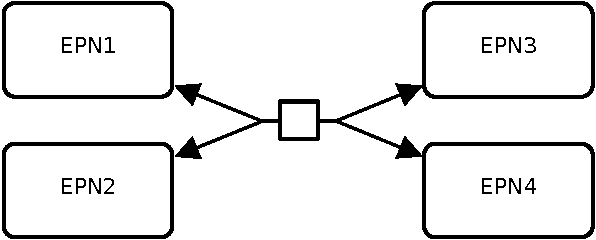
\includegraphics[scale = 0.4]{images/reversible_process}
  \caption{A valid reversible process. A process is reversible if its LHS and RHS contain only \glyph{production} arcs.}
  \label{fig:process-reversibility}
\end{figure}
 
\begin{enumerate}
\item  A mixture of \glyph{consumption} and \glyph{production} arcs on the same side of a \glyph{process} is not permitted.
\item A \glyph{sink} cannot be linked to a reversible process as it only receives entities, and so would effectively make the process irreversible\footnote{A \glyph{source} can only be associated with a \glyph{consumption} arc so this rule does not apply in this case.}.
\item The semantics of \glyph{modulation} is the same as for irreversible processes, .i.e. the amount of entity in the modulation pool affects the rate of the process.
\end{enumerate}

 
\subsection{Cloning}

SBGN allows identical nodes to be duplicated on a map if they are
explicitly marked as such. This is done using a \glyph{clone marker}. The details are shown in table \ref{tab:processduprules}.


\begin{center}
\tablecaption{Duplication rules.}
\label{tab:processduprules}
\begin{footnotesize}
\tablefirsthead{\hline
  Node & Can be duplicated & Indication & Additional Rules\\\hline}
\tablehead{\hline
\multicolumn{4}{|l|}{\small\sl continued from previous page}\\
\hline\hline
  Node & Duplicate? & Indication & Additional Rules\\\hline\hline}
\tabletail{\hline
\multicolumn{4}{|r|}{\small\sl continued on next page}\\
\hline}
\tablelasttail{\hline}
\begin{supertabular}{|l|c|p{4cm}|p{3.5cm}|}\hline
%  Node & Duplicate? & How & Additional Rules\\\hline
Compartment   & N & & \\\hline
SimpleChemical & Y & \glyph{Simple clone marker} & \\\hline
UnspecifiedEntity & Y & \glyph{Simple clone marker} & \\\hline
Source & N & & \\\hline
Sink & N & & \\\hline
Perturbing Agent & Y & \glyph{Simple clone marker} & \\\hline
Phenotype & Y & \glyph{Simple clone marker} & \\\hline
MultimerChemicalEntity & Y & \glyph{Simple clone marker} & \\\hline
StatefulEntityPool & Y & \glyph{Labeled clone marker} & \\\hline
Macromolecule & Y & \glyph{Labeled clone marker} & \\\hline
MultimerMacromolecule & Y & \glyph{Labeled clone marker} & \\\hline
Nucleic\-Acid\-Feature & Y & \glyph{Labeled clone marker} & \\\hline
Complex & Y & \glyph{Labeled clone marker} & \\\hline
Process & Y & None & Duplication is implied when all EPNs linked to the Process are marked as clones.\\\hline
OmittedProcess & Y & As Process  & \\\hline
UncertainProcess & Y & As Process  & \\\hline
Association & Y & As Process  & \\\hline
Dissociation & Y & As Process  & \\\hline
LogicalOperator & Y & None & \\\hline
AND & Y & None & \\\hline
OR & Y & None & \\\hline
NOT & Y & None & \\\hline
\end{supertabular}
\end{footnotesize}
\end{center}


\subsection{Compartment spanning}

An \glyph{EPN} cannot \emph{belong} to more than one
\glyph{compartment}. However, an EPN can be \emph{drawn} over more than one
\glyph{compartment}. In such cases, the decision on which is the owning
\glyph{compartment} is deferred to the drawing tool or the
author. A \glyph{complex} may contain EPNs which belong to different
\glyph{compartments} and in this way a \glyph{complex} can be used to describe
entities that span more than one {compartment}.

This restriction makes it impossible to represent in a semantically
correct way a macromolecule that spans more then one compartment ---
for example a receptor protein. It is clearly desirable to be able to
show a macromolecule in a manner that the biologist expects (i.e.\,
spanning from the outside through the membrane to the
inside). Therefore, the author is recommended to draw the
macromolecule across compartment boundaries, but the underlying SBGN
semantic model will assign it to only one. The assignment to a
\glyph{compartment} may be decided by the software drawing tool or the
author. Note that this has implications for auto-layout algorithms as
they will only be able to treat such \glyph{entity pool nodes} as contained within
a \glyph{compartment} and will have no way of knowing a macromolecule spans a
compartment.

The current solution is consistent with other Systems Biology
representations such as SBML and BioPAX. For more information about the
problems representing membrane spanning proteins and the rationale
behind the current solution see \sect{postponed}.

\subsection{Submaps}

The submap is a visual device that allows the detail of an \PD map to be exported into another \PD map and replaced by a \glyph{submap} glyph, which acts as a place-holder. This is described and illustrated in \sect{submap}. In the following discussion we will refer to the original map as the \emph{main} map and the map containing the export detail as the submap. 

\begin{enumerate}
\item For a valid mapping between an EPN in the map and submap to exist the identifiers in the \glyph{tag} and the submap terminal must be identical and their associated entity pool nodes must be identical.
\item If the same EPN is present in the map and a submap, then they must be mapped to each other.
\item Since the main map and submap share the same namespace, an EPN that is cloned in the main map must also be
marked as cloned in the submap --- even if there is only one copy of the EPN in the submap. The converse applies when the EPN in the submap is cloned\footnote{This has the additional benefit of ensuring that main maps and submaps do not need to be modified if the submap is exanded and collapsed by a viewing or editing tool.}.
\end{enumerate}

% \section{Summary of Rules}

% This section summarises the rules of SBGN-PD in a form that is intended to be accessible to tool developers and those interested in validating process maps. Each rule has been given an identifier for ease of reference. Note that no meaning is attached to the rule identifier and any perceived ordering of the identifiers is not significant.

% \subsection{Entity Pool Nodes}

% \begin{description}
% \item[PD1] The identity of an EPN is defined by a combination of its compartment, entity type (e.g. complex or macromolecule), name and state variables (if any).
% \item[PD2] A Complex’s identity consists of the identity of its subunits and a name is optional. All complexes with the same name should have the same subunits.
% \item[PD3] An EPN may belong to only one compartment.
% \item[PD4] An EPN belongs to only one compartment. If no compartment is draw it is assumed to belong to a “default” compartment.
% \item[PD5] An EPN can overlap more than one compartment and in this case it is deferred to the drawing tool or author to assign the owning compartment. Note this rule need not apply in cases where SBGN is draw by hand.
% \item[PD6] A Complex may contain subunits that belong to different compartments (the complex itself will belong to only one, however).
% \item[PD7] The layout or organisation of a compartment does not imply anything about its topology.
% \item[PD8] The layout or organisation of the EPNs in a complex does not imply any information about topology.
% \item[PD10] Complexes can be nested. This does imply information about the complex’s topology.
% \item[PD11] A complex should consist of different EPNs. If two or more elements of the complex are identical then they should be replaced by a multimer.
% \item[PD12] Source and sink nodes must have no name and be attached to only one consumption or production arc.
% \item[PD13] An EPN must be connected to at least 1 consumption, production or modulation arc.
% \item[PD14] An EPN is not allowed to be a substrate and product of the same process. This applies to cloned EPNs as well.
% States
% \item[PD15] All state variables in a stateful EPN should have different names.
% \item[PD16] A blank state variable has the value “unset”.
% \item[PD17] The state of a complex is the sum of its subunits’ and its own state variables.
% \item[PD48] The \glyph{Sink} cannot be linked to a reversible process.
% \end{description}

% \subsection{Compartments}

% \begin{description}
% \item[PD18] Compartments cannot be nested. Compartments may overlap, but overlap does not imply containment.
% \item[PD19] The layout or organisation of a compartment does not imply anything about its topology.
% \item[PD20] If no compartment is draw it is assumed to belong to a “default” compartment.
% \item[PD21] If one or more compartment glyphs are drawn then all EPNs must owned by a compartment glyph.
% \end{description}

% \subsection{Process Nodes (PN)}

% \begin{description}
% \item[PD22] A Process Node should have non-zero number of consumption and production links.
% \item[PD23] All substrates of the Process Node should be different. If several copies of the same EPN are involved in the process, the cardinality label of consumption arc should be used.
% \item[PD24] All products of the PN should be different. If several copies of the same EPN are produced in the process, the cardinality label of production arc should be used.
% \item[PD25] Once the cardinality label is added to one arc connected to a PN all other such arcs should display a cardinality label.
% \item[PD26] The cardinality of an arc can be undefined or unknown, in which case a question mark (``?'') should be used.
% \item[PD27] A PN should correspond to only one process or series of connected process. The same set of EPNs should be connected by different PNs if they are consumed and produced by different processes.
% \item[PD28] The composition of the products of an association process should be equivalent to its substrates
% \item[PD29] The composition of the products of a dissociation process should be equivalent to its substrate.
% \end{description}

% \subsection{Modulation and Logical Operators}

% \begin{description}
% \item[PD30] A PN with no modulations has an underlying “basal rate” which describes the rate at which it converts inputs to outputs.
% \item[PD31] Modulation changes the basal rate in an unspecified fashion.
% \item[PD32] Stimulation is a modulation that’s effect is to increase the basal rate.
% \item[PD33] Inhibition is a modulation that’s effect is to decrease the basal rate.
% \item[PD34] The above types of modulation, when assigned to the same process are combined and have a multiplicative effect on the basal rate of the process.
% \item[PD35] Modulators that do not interact with each other in the above manner should be drawn as modulating different process nodes. Their effect is therefore additive.
% \item[PD36] At most one trigger can be assigned to a process. Two triggers would imply an implicit Boolean AND or OR operator, so for clarity only one trigger can be assigned to a process and such combinations must be explicitly expressed as the Boolean operators.
% \item[PD37] The PN should have only one Catalysis arc connected to it. A catalysis modulation implies that the exact biochemical mechanism underlying the process is known.
% \item[PD38] The PN should have only one Trigger arc connected to it.
% \item[PD39] AND and OR Boolean logic gates should have two or more input and one output.
% \item[PD40] A NOT gate can only have one input and output.
% \end{description}

% \subsection{Cloning and Sub-Maps}

% \begin{description}
% \item[PD41] Duplicate EPNs must be marked as clones.
% \item[PD42] Duplicate stateful EPNs must use a Labelled Clone Marker.
% \item[PD43] Duplicate non-stateful EPNs must use a simple clone marker.
% \item[PD44] A sub-map shares the same namespace as its main map.
% \item[PD45] To map an EPN in the main map to one in a sub-map, the SubMap glyph in the main map must contain an identifier that matches the identifier of a Tag in the sub-map. Both EPNs must be identical.
% \item[PD46] If a main map and a sub-map contain an identical EPN then a mapping must exist between them.
% \item[PD47] If an EPN is cloned in the main map, then it must be marked as cloned in the sub-map, with the same identifier in both maps. This is true if there is only one EPN of this type in the submap.
% \end{description}

